A few notes before starting this assignment:

I'm considering four frames. 

The first one is the inertial frame. It is in A with the first axis straight up, the second right and the third into the plane of the image.

\begin{figure}[ht]
    \centering
    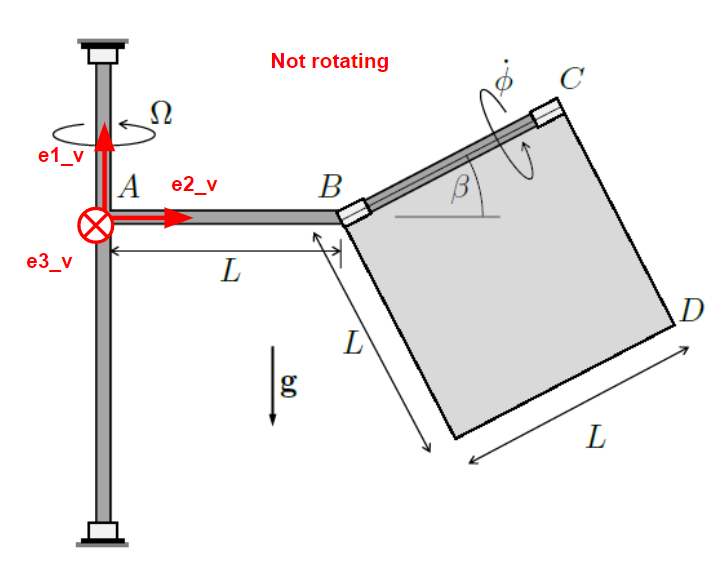
\includegraphics[scale=0.5]{images/inertial_frame.png}
    \caption{Inertial Frame}
    %label always in the end
    \label{fig:inertial_frame}
\end{figure}

\noindent The second one is located at the same position but rotating with Omega. I will call it the vertical frame.

\begin{figure}[ht]
    \centering
    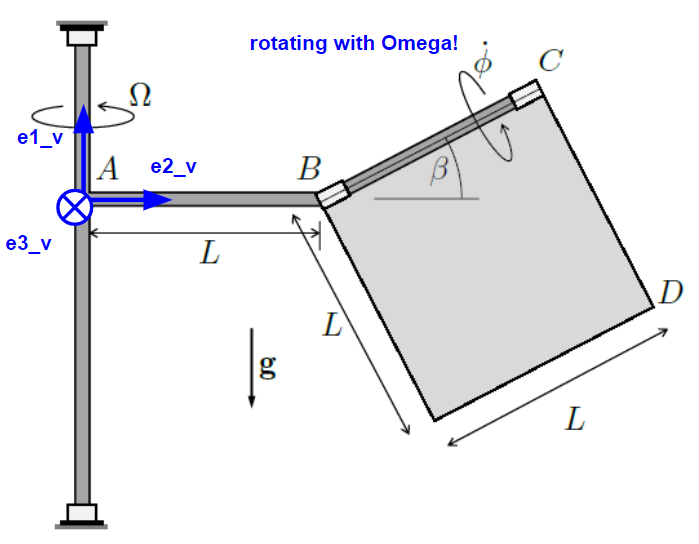
\includegraphics[scale=0.5]{images/vertical_frame.png}
    \caption{Vertical Frame}
    %label always in the end
    \label{fig:vertical_frame}
\end{figure}
\clearpage %HERE

The third one, that is called rod frame is located in the point B and relative to the vertical frame it is tilted by $\beta$ around the positive $e_3^v$ axis.

\begin{figure}[ht]
    \centering
    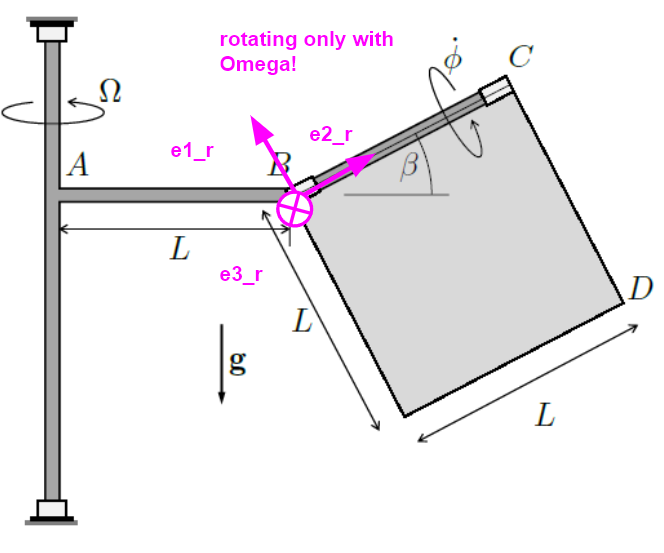
\includegraphics[scale=0.5]{images/rod_frame.png}
    \caption{Rod Frame}
    %label always in the end
    \label{fig:rod_frame}
\end{figure}

The last frame is the square frame which relative to the rod frame is also rotation with $\phi$:

\begin{figure}[ht]
    \centering
    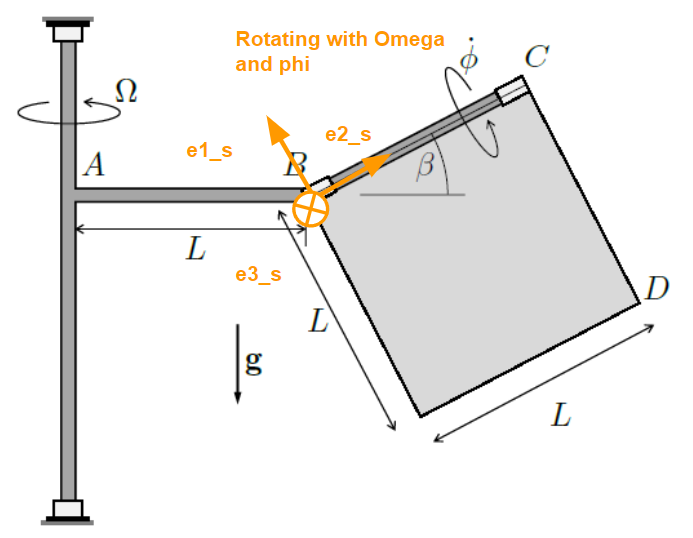
\includegraphics[scale=0.5]{images/square_frame.png}
    \caption{Square Frame}
    %label always in the end
    \label{fig:square_frame}
\end{figure}


\subsection{Kinetic and Potential Energy}
\subsubsection{Vertical Shaft}
As the vertical bar rotates around the thin axis and is static regarding the height of it's CoM the contribution to the energy is 0.

\begin{equation}
    \begin{split}
        T_\text{vertical bar} =  V_\text{vertical bar} = 0
    \end{split}
\end{equation}
\subsubsection{Horizontal Bar}
\textbf{Note: } I will refer to the horizontal bar as bar and to the tilted bar as rod.

As point A which is part of the bar is not moving we can simply consider the rotational part w.r.t. to this fixed point A.:

\begin{equation}
    \begin{split}
        T_\text{bar} =  \frac{L^2\Omega ^2m}{6}
    \end{split}
\end{equation}

As the bar is horizontal on the height of A we have no contribution of the potential energy.

\begin{equation}
    \begin{split}
        V_\text{bar} = 0
    \end{split}
\end{equation}

\subsubsection{Rod}
As the rod has no static point we will use a superposition of the rotational and translational kinetic energy.

\begin{equation}
    \begin{split}
        T_\text{Rod transl} = \frac{L^2\Omega ^2m{\left(\cos\left(\beta \right)+2\right)}^2}{8}
    \end{split}
\end{equation}
For the rotational part considering the moment of inertia of the center of mass we get:
\begin{equation}
    \begin{split}
        T_\text{Rod rot} = \frac{L^2\Omega ^2m{\cos\left(\beta \right)}^2}{24}
    \end{split}
\end{equation}
Which leads to:
\begin{equation}
    \begin{split}
        \Rightarrow T_\text{Rod} = \frac{L^2\Omega ^2m\left({\cos\left(\beta \right)}^2+3\cos\left(\beta \right)+3\right)}{6}
    \end{split}
\end{equation}

For the potential energy we have the verical part of the incline of the rod:

\begin{equation}
    \begin{split}
        V_\text{Rod} = \frac{L}{2}mg\sin\beta
    \end{split}
\end{equation}

\subsubsection{Square Plate}
As for the rod, first the translational kinetic energy:

\begin{equation}
    \begin{split}
        T_\text{square transl} = &\frac{M}{2}\left(\left(\vphantom{\int}\left(\Omega +\mathrm{\dot\phi}\sin\left(\beta \right)\right)\left(\frac{L\left(\sin\left(\Omega t\right)\sin\left(\phi \right)-\cos\left(\Omega t\right)\cos\left(\phi \right)\sin\left(\beta \right)\right)}{2}-\frac{L\cos\left(\Omega t\right)\cos\left(\beta \right)}{2}\right)\right.\right.\\
        &\left.-L\Omega \cos\left(\Omega t\right)+\frac{L\mathrm{\dot\phi}\cos\left(\Omega t\right)\cos\left(\beta \right)\left(\sin\left(\beta \right)-\cos\left(\beta \right)\cos\left(\phi \right)\right)}{2}\right)^2\\
        &+\left(\left(\Omega +\mathrm{\dot\phi}\sin\left(\beta \right)\right)\left(\frac{L\left(\cos\left(\Omega t\right)\sin\left(\phi \right)+\sin\left(\Omega t\right)\cos\left(\phi \right)\sin\left(\beta \right)\right)}{2}+\frac{L\sin\left(\Omega t\right)\cos\left(\beta \right)}{2}\right)\right.\\
        &\left.\left.+L\Omega \sin\left(\Omega t\right)-\frac{L\mathrm{\dot\phi}\sin\left(\Omega t\right)\cos\left(\beta \right)\left(\sin\left(\beta \right)-\cos\left(\beta \right)\cos\left(\phi \right)\right)}{2}\right)^2+\frac{L^2{\mathrm{\dot\phi}}^2{\cos\left(\beta \right)}^2{\sin\left(\phi \right)}^2}{4}\right)
    \end{split}
\end{equation}

For the rotational part we get, considering the moment of inertia w.r.t. the c.o.m. in the s frame:

\begin{equation}
    \begin{split}
        T_\text{square rot} = &\frac{L^2M\left(\mathrm{\dot\phi}+\Omega \sin\left(\beta \right)\right)\left(\frac{\mathrm{\dot\phi}}{2}+\frac{\Omega \sin\left(\beta \right)}{2}\right)}{12}\\
        &+\frac{L^2M\Omega ^2{\cos\left(\beta \right)}^2{\cos\left(\phi \right)}^2}{24}
    \end{split}
\end{equation}

Which leads to:

\begin{equation}
    \begin{split}
        T_\text{square} = &\frac{L^2M}{12}\left(-\Omega ^2{\cos\left(\beta \right)}^2{\cos\left(\phi \right)}^2+\Omega ^2{\cos\left(\beta \right)}^2\right.\\
        &+3\sin\left(\beta \right)\Omega ^2\cos\left(\beta \right)\cos\left(\phi \right)+6\Omega ^2\cos\left(\beta \right)\\
        &+6\sin\left(\beta \right)\Omega ^2\cos\left(\phi \right)+8\Omega ^2+3\Omega \mathrm{\dot\phi}\cos\left(\beta \right)\cos\left(\phi \right)\\
        &\left.\vphantom{\int}+6\Omega \mathrm{\dot\phi}\cos\left(\phi \right)+4\sin\left(\beta \right)\Omega \mathrm{\dot\phi}+2{\mathrm{\dot\phi}}^2\right)
    \end{split}
\end{equation}

For the potential energy we get:
\begin{equation}
    \begin{split}
        \frac{L}{2}Mg\left(\sin\left(\beta \right)-\cos\left(\beta \right)\cos\left(\phi \right)\right)
    \end{split}
\end{equation}

Which are the contributions of the vertical parts of the two vectors of length $\frac{L}{2}$ to the center of mass of the square in the s frame. The sin part points up (to c.o.m of the rod) and the cos part points down.

\subsubsection{Total Energy}
The total kinetic energy comes to:

\begin{equation}
    \begin{split}
        &T = \underbrace{T_\text{vertical bar}}_{0} + T_\text{bar} + T_\text{Rod} + T_\text{Square} = \\
        &\frac{L^2}{12}\left(8M\Omega ^2+8\Omega ^2m+2M{\mathrm{\dot\phi}}^2+6M\Omega ^2\cos\left(\beta \right)+6\Omega ^2m\cos\left(\beta \right)\right.\\
        &+M\Omega ^2{\cos\left(\beta \right)}^2+2\Omega ^2m{\cos\left(\beta \right)}^2+6M\Omega ^2\cos\left(\phi \right)\sin\left(\beta \right)\\
        &+6M\Omega \mathrm{\dot\phi}\cos\left(\phi \right)+4M\Omega \mathrm{\dot\phi}\sin\left(\beta \right)-M\Omega ^2{\cos\left(\beta \right)}^2{\cos\left(\phi \right)}^2\\
        &\left.\vphantom{\int}+3M\Omega \mathrm{\dot\phi}\cos\left(\beta \right)\cos\left(\phi \right)+3M\Omega ^2\cos\left(\beta \right)\cos\left(\phi \right)\sin\left(\beta \right)\right)
    \end{split}
\end{equation}

Analogous the potential energy:
\begin{equation}
    \begin{split}
        &V = \underbrace{V_\text{vertical bar}}_{0} + V_\text{bar} + V_\text{Rod} + V_\text{Square} = \\
        & \frac{L}{2}Mg\left(2\sin\left(\beta \right)-\cos\left(\beta \right)\cos\left(\phi \right)\right)
    \end{split}
\end{equation}

Where one can see nicely the double contribution of the c.o.m of the rod for the rod and the square and the negative part of the square.


\subsection{Lagrange Equations}
Having an expression for the kinetic and potential energy we can use them to denote our lagrange equations:

\begin{equation}
    \begin{split}
        \frac{\partial}{\partial t}\frac{\partial T}{\partial \dot\phi} - \frac{\partial T}{\partial \phi} + \frac{\partial V}{\partial \phi} = 0
    \end{split}
\end{equation}

Which yields:

\begin{equation}
    \begin{split}
        &\frac{LM}{12}\left(-2L\cos\left(\phi \right)\sin\left(\phi \right)\Omega ^2{\cos\left(\beta \right)}^2+3L\sin\left(\beta \right)\sin\left(\phi \right)\Omega ^2\cos\left(\beta \right)\right.\\
        &\left.\vphantom{\int}+6L\sin\left(\beta \right)\sin\left(\phi \right)\Omega ^2+6g\sin\left(\phi \right)\cos\left(\beta \right)+4L\mathrm{\ddot\phi}\right) = 0
    \end{split}
\end{equation}

Which is a differential equation for $\phi$.

\subsection{Non constant angular velocity around vertical Shaft}
\subsubsection{Vertical shaft}
Unchanged
\subsubsection{Bar}

 \begin{equation}
    \begin{split}
        T_\text{bar} = \frac{L^2\Omega ^2m}{6}
    \end{split}
 \end{equation}

 \begin{equation}
    \begin{split}
        V_\text{bar} = 0
    \end{split}
 \end{equation}

 \subsubsection{Rod}

 \begin{equation}
    \begin{split}
        T_\text{rod} = L^2m\mathrm{\dot\theta}^2\left(\frac{\cos\left(\beta \right)^2}{2}+\cos\left(\beta \right)+1\right)
    \end{split}
 \end{equation}

 \begin{equation}
    \begin{split}
        V_\text{rod} = \frac{L}{2}gm\sin\left(\beta \right)
    \end{split}
 \end{equation}

 \subsubsection{Square}

 \begin{equation}
    \begin{split}
        T_\text{square} = &\frac{L^2M}{12}\left(2{\mathrm{\dot\phi}}^2+3\mathrm{\dot\phi}\mathrm{\dot\theta}\cos\left(\beta \right)\cos\left(\phi \right)+6\mathrm{\dot\phi}\mathrm{\dot\theta}\cos\left(\phi \right)+4\sin\left(\beta \right)\mathrm{\dot\phi}\mathrm{\dot\theta}\right.\\
        &-{\mathrm{\dot\theta}}^2{\cos\left(\beta \right)}^2{\cos\left(\phi \right)}^2+{\mathrm{\dot\theta}}^2{\cos\left(\beta \right)}^2+3\sin\left(\beta \right){\mathrm{\dot\theta}}^2\cos\left(\beta \right)\cos\left(\phi \right)\\
        &\left.\vphantom{\int}+6{\mathrm{\dot\theta}}^2\cos\left(\beta \right)+6\sin\left(\beta \right){\mathrm{\dot\theta}}^2\cos\left(\phi \right)+8{\mathrm{\dot\theta}}^2\right)
    \end{split}
 \end{equation}

 \begin{equation}
    \begin{split}
        V_\text{square} = \frac{L}{2}Mg\left(\sin\left(\beta \right)-\cos\left(\beta \right)\cos\left(\phi \right)\right)
    \end{split}
 \end{equation}

 \subsubsection{Total Energy}

 \begin{equation}
    \begin{split}
        T = &\frac{L^2}{12}\left(2M{\mathrm{\dot\phi}}^2+8M{\mathrm{\dot\theta}}^2+8m{\mathrm{\dot\theta}}^2+6M{\mathrm{\dot\theta}}^2\cos\left(\beta \right)+6m{\mathrm{\dot\theta}}^2\cos\left(\beta \right)\right.\\
        &+M{\mathrm{\dot\theta}}^2{\cos\left(\beta \right)}^2+2m{\mathrm{\dot\theta}}^2{\cos\left(\beta \right)}^2+6M{\mathrm{\dot\theta}}^2\cos\left(\phi \right)\sin\left(\beta \right)\\
        &+6M\mathrm{\dot\phi}\mathrm{\dot\theta}\cos\left(\phi \right)+4M\mathrm{\dot\phi}\mathrm{\dot\theta}\sin\left(\beta \right)-M{\mathrm{\dot\theta}}^2{\cos\left(\beta \right)}^2{\cos\left(\phi \right)}^2\\
        &\left.\vphantom{\int}+3M\mathrm{\dot\phi}\mathrm{\dot\theta}\cos\left(\beta \right)\cos\left(\phi \right)+3M{\mathrm{\dot\theta}}^2\cos\left(\beta \right)\cos\left(\phi \right)\sin\left(\beta \right)\right)
    \end{split}
 \end{equation}

 \begin{equation}
    \begin{split}
        V = \frac{L}{2}gm\sin\left(\beta \right)+\frac{L}{2}Mg\left(\sin\left(\beta \right)-\cos\left(\beta \right)\cos\left(\phi \right)\right)
    \end{split}
 \end{equation}

 \subsubsection{Lagrange Equations}

%  As now we have two generalized coordinates we also have two lagrangr equations. For $\phi$ we get:

%  \begin{equation}
%     \begin{split}
%         &\frac{LM}{12}\left(-2L\cos\left(\phi \right)\sin\left(\phi \right){\mathrm{\dot\theta}}^2{\cos\left(\beta \right)}^2+3L\sin\left(\beta \right)\sin\left(\phi \right){\mathrm{\dot\theta}}^2\cos\left(\beta \right)\right.\\
%         &\left.\vphantom{\int}+6L\sin\left(\beta \right)\sin\left(\phi \right){\mathrm{\dot\theta}}^2+6g\sin\left(\phi \right)\cos\left(\beta \right)+4L\mathrm{\ddot\phi}\right)
%     \end{split}
%  \end{equation}

%  And for $\theta$:

%  \begin{equation}
%     \begin{split}
%         &\frac{L^2}{12}\mathrm{\ddot\theta}\left(16M+16m+12M\cos\left(\beta \right)+12m\cos\left(\beta \right)+2M{\cos\left(\beta \right)}^2\right.\\
%         &+4m{\cos\left(\beta \right)}^2-2M{\cos\left(\beta \right)}^2{\cos\left(\phi \right)}^2+12M\cos\left(\phi \right)\sin\left(\beta \right)\\
%         &\left.\vphantom{\int}+6M\cos\left(\beta \right)\cos\left(\phi \right)\sin\left(\beta \right)\right)
%     \end{split}
%  \end{equation}

As we have now two generalized coordinates the lagrange equations look like this:

\begin{equation}
    \begin{split}
        \frac{\partial}{\partial t}\frac{\partial T}{\partial  \text{\textbf{q}}} - \frac{\partial T}{\partial \text{\textbf{q}}} + \frac{\partial V}{\partial \text{\textbf{q}}} = 0
    \end{split}
\end{equation}

Where $\text{\textbf{q}} = \begin{pmatrix}
    \phi\\
    \theta
\end{pmatrix}$

This leads to two equations. For visualization purposes I will write down the entries one after the other:

\begin{equation}
    \begin{split}
        &\frac{L^2\,M\,\mathrm{\ddot \phi}}{3}+\frac{L^2\,M\,\mathrm{\ddot  \theta}\,\left(6\,\cos\left(\phi \right)+4\,\sin\left(\beta \right)+3\,\cos\left(\beta \right)\,\cos\left(\phi \right)\right)}{12}+\frac{L\,M\,g\,\cos\left(\beta \right)\,\sin\left(\phi \right)}{2}\\
        &+\frac{L^2\,M\,\mathrm{\dot  \theta}\,\sin\left(\phi \right)\,\left(6\,\mathrm{\dot \phi}+3\,\mathrm{\dot \phi}\,\cos\left(\beta \right)+6\,\mathrm{\dot  \theta}\,\sin\left(\beta \right)+3\,\mathrm{\dot  \theta}\,\cos\left(\beta \right)\,\sin\left(\beta \right)-2\,\mathrm{\dot  \theta}\,{\cos\left(\beta \right)}^2\,\cos\left(\phi \right)\right)}{12}\\
        &-\frac{L^2\,M\,\mathrm{\dot \phi}\,\mathrm{\dot  \theta}\,\sin\left(\phi \right)\,\left(\cos\left(\beta \right)+2\right)}{4}
    \end{split}
\end{equation}

And

\begin{equation}
    \begin{split}
        &\frac{L^2\,\mathrm{\ddot  \theta}}{12}\,\left(\vphantom{\int}16\,M+16\,m+12\,M\,\cos\left(\beta \right)+12\,m\,\cos\left(\beta \right)+2\,M\,{\cos\left(\beta \right)}^2\right.\\
        &\left.\vphantom{\int}+4\,m\,{\cos\left(\beta \right)}^2-2\,M\,{\cos\left(\beta \right)}^2\,{\cos\left(\phi \right)}^2+12\,M\,\cos\left(\phi \right)\,\sin\left(\beta \right)+6\,M\,\cos\left(\beta \right)\,\cos\left(\phi \right)\,\sin\left(\beta \right)\right)\\
        &+\frac{L^2\,M\,\mathrm{\ddot \phi}\,\left(6\,\cos\left(\phi \right)+4\,\sin\left(\beta \right)+3\,\cos\left(\beta \right)\,\cos\left(\phi \right)\right)}{12}\\
        &-\frac{L^2\,M\,\mathrm{\dot \phi}\,\sin\left(\phi \right)\,\left(6\,\mathrm{\dot \phi}+3\,\mathrm{\dot \phi}\,\cos\left(\beta \right)+12\,\mathrm{\dot  \theta}\,\sin\left(\beta \right)+6\,\mathrm{\dot  \theta}\,\cos\left(\beta \right)\,\sin\left(\beta \right)-4\,\mathrm{\dot  \theta}\,{\cos\left(\beta \right)}^2\,\cos\left(\phi \right)\right)}{12}
    \end{split}
\end{equation}



\subsection{Non Conservative Forces}\label{subsec:3.4}
Now we have a non conservative force attacking on the square.

We have to derive the velocity of a random point on the square. In the following I will parametrize said point with $x_1$ and $x_2$ which are the coordinates of the point on the square in the s frame from B.

\begin{equation}
    \begin{split}
        v_{Pi} &= v_{Bi} + \omega_i \times BP_i
        % \\&=\begin{pmatrix}
        %     &-\mathrm{\dot\phi}x_{1}\cos\left(\beta \right)\sin\left(\phi \right)\\
        %     &\left(x_{1}\left(\cos\left(\theta \right)\sin\left(\phi \right)+\cos\left(\phi \right)\sin\left(\beta \right)\sin\left(\theta \right)\right)-x_{2}\cos\left(\beta \right)\sin\left(\theta \right)\right)\left(\mathrm{\dot\theta}+\mathrm{\dot\phi}\sin\left(\beta \right)\right)-L\mathrm{\dot\theta}\sin\left(\theta \right)+\mathrm{\dot\phi}\cos\left(\beta \right)\sin\left(\theta \right)\left(x_{2}\sin\left(\beta \right)+x_{1}\cos\left(\beta \right)\cos\left(\phi \right)\right)\\
        %     &\left(x_{1}\left(\sin\left(\phi \right)\sin\left(\theta \right)-\cos\left(\phi \right)\sin\left(\beta \right)\cos\left(\theta \right)\right)+x_{2}\cos\left(\beta \right)\cos\left(\theta \right)\right)\left(\mathrm{\dot\theta}+\mathrm{\dot\phi}\sin\left(\beta \right)\right)+L\mathrm{\dot\theta}\cos\left(\theta \right)-\mathrm{\dot\phi}\cos\left(\beta \right)\cos\left(\theta \right)\left(x_{2}\sin\left(\beta \right)+x_{1}\cos\left(\beta \right)\cos\left(\phi \right)\right)
        % \end{pmatrix}
    \end{split}
\end{equation}

Therefore the work of the force contribution at a single point P is:

\begin{equation}
    \begin{split}
        dW = &-cvP_i\bullet vP_i = \\
        &= -c\left(\vphantom{\int}\left(\vphantom{\sum}x_{1}\left(\sin\left(\phi \right)\sin\left(\theta \right)-\cos\left(\phi \right)\sin\left(\beta \right)\cos\left(\theta \right)\right)\right.\right.\\
        &\left.\vphantom{\sum}+x_{2}\cos\left(\beta \right)\cos\left(\theta \right)\right)\left(\mathrm{\dot\theta}+\mathrm{\dot\phi}\sin\left(\beta \right)\right)+L\mathrm{\dot\theta}\cos\left(\theta \right)\\
        &\left.\vphantom{\int}-\mathrm{\dot\phi}\cos\left(\beta \right)\cos\left(\theta \right)\left(x_{2}\sin\left(\beta \right)+x_{1}\cos\left(\beta \right)\cos\left(\phi \right)\right)\right)^2\\
        &-c\left(\vphantom{\int}\left(\vphantom{\sum}x_{1}\left(\cos\left(\theta \right)\sin\left(\phi \right)+\cos\left(\phi \right)\sin\left(\beta \right)\sin\left(\theta \right)\right)-x_{2}\cos\left(\beta \right)\sin\left(\theta \right)\right)\right.\\
&\left(\mathrm{\dot\theta}+\mathrm{\dot\phi}\sin\left(\beta \right)\right)-L\mathrm{\dot\theta}\sin\left(\theta \right)\\
&\left.\vphantom{\sum}+\mathrm{\dot\phi}\cos\left(\beta \right)\sin\left(\theta \right)\left(x_{2}\sin\left(\beta \right)+x_{1}\cos\left(\beta \right)\cos\left(\phi \right)\vphantom{\sum}\right)\vphantom{\int}\right)^2\\
&-c{\mathrm{\dot\phi}}^2{x_{1}}^2{\cos\left(\beta \right)}^2\sin\left(\phi \right)^2
    \end{split}
\end{equation}

As we want to derive the whole work done by the area distributed force we integrate the expression of dW over the whole square:

\begin{equation}
    \begin{split}
        W = &\int_{x_1 = -L}^0\int_{x_2 = 0}^L-c\left(\vphantom{\int}\left(\vphantom{\sum}x_{1}\left(\sin\left(\phi \right)\sin\left(\theta \right)-\cos\left(\phi \right)\sin\left(\beta \right)\cos\left(\theta \right)\right)\right.\right.\\
        &\left.\vphantom{\sum}+x_{2}\cos\left(\beta \right)\cos\left(\theta \right)\right)\left(\mathrm{\dot\theta}+\mathrm{\dot\phi}\sin\left(\beta \right)\right)+L\mathrm{\dot\theta}\cos\left(\theta \right)\\
        &\left.\vphantom{\int}-\mathrm{\dot\phi}\cos\left(\beta \right)\cos\left(\theta \right)\left(x_{2}\sin\left(\beta \right)+x_{1}\cos\left(\beta \right)\cos\left(\phi \right)\right)\right)^2\\
        &-c\left(\vphantom{\int}\left(\vphantom{\sum}x_{1}\left(\cos\left(\theta \right)\sin\left(\phi \right)+\cos\left(\phi \right)\sin\left(\beta \right)\sin\left(\theta \right)\right)-x_{2}\cos\left(\beta \right)\sin\left(\theta \right)\right)\right.\\
&\left(\mathrm{\dot\theta}+\mathrm{\dot\phi}\sin\left(\beta \right)\right)-L\mathrm{\dot\theta}\sin\left(\theta \right)\\
&\left.\vphantom{\sum}+\mathrm{\dot\phi}\cos\left(\beta \right)\sin\left(\theta \right)\left(x_{2}\sin\left(\beta \right)+x_{1}\cos\left(\beta \right)\cos\left(\phi \right)\vphantom{\sum}\right)\vphantom{\int}\right)^2\\
&-c{\mathrm{\dot\phi}}^2{x_{1}}^2{\cos\left(\beta \right)}^2\sin\left(\phi \right)^2dx_2dx_1
    \end{split}
\end{equation}

Which comes to:

\begin{equation}
    \begin{split}
        W = &-\frac{cL^4{\mathrm{\dot\phi}}^2}{3}-\frac{cL^4\mathrm{\dot\phi}\mathrm{\dot\theta}\cos\left(\beta \right)\cos\left(\phi \right)}{2}-cL^4\mathrm{\dot\phi}\mathrm{\dot\theta}\cos\left(\phi \right)-\\
        &\frac{2c\sin\left(\beta \right)L^4\mathrm{\dot\phi}\mathrm{\dot\theta}}{3}+\frac{cL^4{\mathrm{\dot\theta}}^2{\cos\left(\beta \right)}^2{\cos\left(\phi \right)}^2}{3}-\frac{cL^4{\mathrm{\dot\theta}}^2{\cos\left(\beta \right)}^2}{3}-\\
        &\frac{c\sin\left(\beta \right)L^4{\mathrm{\dot\theta}}^2\cos\left(\beta \right)\cos\left(\phi \right)}{2}-cL^4{\mathrm{\dot\theta}}^2\cos\left(\beta \right)-c\sin\left(\beta \right)L^4{\mathrm{\dot\theta}}^2\cos\left(\phi \right)\\
        &-\frac{4cL^4{\mathrm{\dot\theta}}^2}{3}
    \end{split}
\end{equation}

And finally the generalized forces are:

\begin{equation}
    \begin{split}
        Q_\phi = \frac{\partial W}{\partial \phi} = -\frac{L^4c\left(4\mathrm{\dot\phi}+6\mathrm{\dot\theta}\cos\left(\phi \right)+4\mathrm{\dot\theta}\sin\left(\beta \right)+3\mathrm{\dot\theta}\cos\left(\beta \right)\cos\left(\phi \right)\right)}{6}
    \end{split}
\end{equation}

And 

\begin{equation}
    \begin{split}
        Q_\theta = &-\frac{L^4c}{6}\left(\vphantom{\int}16\mathrm{\dot\theta}+12\mathrm{\dot\theta}\cos\left(\beta \right)+6\mathrm{\dot\phi}\cos\left(\phi \right)+4\mathrm{\dot\phi}\sin\left(\beta \right)+4\mathrm{\dot\theta}{\cos\left(\beta \right)}^2\right.\\
        &-4\mathrm{\dot\theta}{\cos\left(\beta \right)}^2{\cos\left(\phi \right)}^2+3\mathrm{\dot\phi}\cos\left(\beta \right)\cos\left(\phi \right)+12\mathrm{\dot\theta}\cos\left(\phi \right)\sin\left(\beta \right)\\
        &\left.\vphantom{\int}+6\mathrm{\dot\theta}\cos\left(\beta \right)\cos\left(\phi \right)\sin\left(\beta \right)\right)
    \end{split}
\end{equation}

\subsection{Values plugged in}
We plug in the values:
\begin{equation}
    \begin{split}
        L=0.25,\beta = \pi/6, M= 0.5, m = 0.2, g = 9.81, c = 0.1
    \end{split}
\end{equation}
\subsection{Equilibrium}
In the equilibrium configuration we have

\begin{equation}
    \begin{split}
        \ddot \phi = \dot \phi = 0, \quad \phi = \phi_\text{eq}
    \end{split}
\end{equation}

And

\begin{equation}
    \begin{split}
        \ddot \theta = \dot \theta = 0, \quad \theta = \theta_\text{eq}
    \end{split}
\end{equation}

For the rheonomic system with a constant Omega and the plugged in values we get:

\begin{equation}\label{eq:3.6.3}
    \begin{split}
        \frac{981\sqrt{3}\sin\left(\phi \right)}{3200}+\frac{\Omega ^2\sin\left(\phi \right)}{128}+\frac{\sqrt{3}\Omega ^2\sin\left(\phi \right)}{512}-\frac{\Omega ^2\cos\left(\phi \right)\sin\left(\phi \right)}{256} = 0
    \end{split}
\end{equation}

Or for the case of a free rotation around A:

\begin{equation}\label{eq:3.6.4}
    \begin{split}
        \left(\begin{array}{c} \frac{981\,\sqrt{3}\,\sin\left(\phi _{\mathrm{eq}}\right)}{3200}\\ 0 \end{array}\right) = \left(\begin{array}{c}0\\ 0 \end{array}\right)
    \end{split}
\end{equation}

And as can be seen the above equation (\ref{eq:3.6.4}) can be read as:

\begin{equation}\label{eq:3.6.5}
    \begin{split}
        \begin{pmatrix}
            A\sin(\phi_{\text{eq}})\\0
        \end{pmatrix} = \begin{pmatrix}
            0\\0
        \end{pmatrix}
    \end{split}
\end{equation}

With a constant A. Which yields 
\begin{equation}
    \begin{split}
        \phi_{\text{eq}} = n*\pi, \quad \text{ for } n = 0,1,2...
    \end{split}
\end{equation}

% \subsubsection{$\phi$ - Equilibrium}

% From equation (\ref{eq:3.6.3}) we can see that the term $\sin\phi$ is present in every part of the expression so that we can say the equilibrium holds for $\phi = n*\pi$, for $n = 0,1,2,...$

This makes sense as $\phi = n*\pi$ describes states where the square plate stays vertical. As we are not considering aerial drag (non-conservative forces) it is imaginable that this is an equilibrium. $\theta$ can be chosen arbitrarily which makes sense as the system is symmetric w.r.t. theta.

\textbf{Note:} as for this case we have a scleronomic system we could have also just used the following:
\begin{equation}
    \begin{split}
        \frac{\partial V}{\partial \text{\textbf{q}}} = \text{\textbf{0}}
    \end{split}
\end{equation}

Which when plugging it in gives us:
\begin{equation}
    \left(\begin{array}{cc} \frac{981\,\sqrt{3}\,\sin\left(\phi _{\mathrm{eq}}\right)}{3200} & 0 \end{array}\right) = \text{\textbf{0}}
\end{equation}

Which is the same as equation (\ref{eq:3.6.4})
% The same holds for a free rotation around A as can bee seen in equation (\ref{eq:3.6.4}).
% \subsubsection{$\theta$ - Equilibrium}

% Solving equation (\ref{eq:3.6.5}) we can see that $\ddot \theta$ has to be 0 and we thus recover a constant angular velocity around A. This makes sense as a constant, unconstrained velocity doesn't generate any forces. Note that if we considered the non-conservative forces from step \ref{subsec:3.4} that the equilibrium would be different.

% \begin{equation}
%     \begin{split}
%         \begin{pmatrix} &\frac{L^2M\mathrm{\ddot \phi}}{3}+\frac{L^2M\mathrm{\ddot \theta}\left(6\cos\left(\phi \right)+4\sin\left(\beta \right)+3\cos\left(\beta \right)\cos\left(\phi \right)\right)}{12}+\frac{LMg\cos\left(\beta \right)\sin\left(\phi \right)}{2}+\frac{L^2M\mathrm{\dot \theta}\sin\left(\phi \right)\left(6\mathrm{\dot \phi}+3\mathrm{\dot \phi}\cos\left(\beta \right)+6\mathrm{\dot \theta}\sin\left(\beta \right)+3\mathrm{\dot \theta}\cos\left(\beta \right)\sin\left(\beta \right)-2\mathrm{\dot \theta}{\cos\left(\beta \right)}^2\cos\left(\phi \right)\right)}{12}-\frac{L^2M\mathrm{\dot \phi}\mathrm{\dot \theta}\sin\left(\phi \right)\left(\cos\left(\beta \right)+2\right)}{4}\\ 
%             &\frac{L^2\mathrm{\ddot \theta}\left(16M+16m+12M\cos\left(\beta \right)+12m\cos\left(\beta \right)+2M{\cos\left(\beta \right)}^2+4m{\cos\left(\beta \right)}^2-2M{\cos\left(\beta \right)}^2{\cos\left(\phi \right)}^2+12M\cos\left(\phi \right)\sin\left(\beta \right)+6M\cos\left(\beta \right)\cos\left(\phi \right)\sin\left(\beta \right)\right)}{12}+\frac{L^2M\mathrm{\ddot \phi}\left(6\cos\left(\phi \right)+4\sin\left(\beta \right)+3\cos\left(\beta \right)\cos\left(\phi \right)\right)}{12}-\frac{L^2M\mathrm{\dot \phi}\sin\left(\phi \right)\left(6\mathrm{\dot \phi}+3\mathrm{\dot \phi}\cos\left(\beta \right)+12\mathrm{\dot \theta}\sin\left(\beta \right)+6\mathrm{\dot \theta}\cos\left(\beta \right)\sin\left(\beta \right)-4\mathrm{\dot \theta}{\cos\left(\beta \right)}^2\cos\left(\phi \right)\right)}{12} \end{pmatrix}
%     \end{split}
% \end{equation}

Lastly when considering the non-conservative forces as well we get:

\begin{equation}
    \begin{split}
        \left(\begin{array}{c} \frac{981\,\sqrt{3}\,\sin\left(\phi _{\mathrm{eq}}\right)}{3200}\\ 0 \end{array}\right)
    \end{split}
\end{equation}

Which is the same equilibrium configuration as for the case with the free rotation of the vertical shaft.
\clearpage
%\HERE
Looking at the equations of motion for the case of constant rotation around the vertical shaft whilst considering the non-conservative forces:

\begin{equation}
    \begin{split}
        &\frac{\Omega }{7680}+\frac{\Omega \,\cos\left(\phi _{\mathrm{eq}}\right)}{2560}+\frac{981\,\sqrt{3}\,\sin\left(\phi _{\mathrm{eq}}\right)}{3200}+\frac{\Omega ^2\,\sin\left(\phi _{\mathrm{eq}}\right)}{128}+\frac{\sqrt{3}\,\Omega ^2\,\sin\left(\phi _{\mathrm{eq}}\right)}{512}\\
        &-\frac{\Omega ^2\,\cos\left(\phi _{\mathrm{eq}}\right)\,\sin\left(\phi _{\mathrm{eq}}\right)}{256}+\frac{\sqrt{3}\,\Omega \,\cos\left(\phi _{\mathrm{eq}}\right)}{10240} = 0
    \end{split}
\end{equation}

From the first view we can see that $\phi = 0$ is not the solution anymore which makes sense because the non-conservative forces simulate aerial drag which would induce a tilt in the square when rotating at a constant angular velocity.

Trying to solve this equation yielded no solution for $\phi_{eq}$. This can be interpreted as follows: We have a constant angular velocity around the vertical shaft. This rotation induces a velocity in the bar, the rod and the square plate. This generates a drag force on the square plate which will remain there as long as there is an angular velocity and therefore no equilibrium can be reached.



\subsection{Integration}

To perform the time integration of the state space representation we use the same approach as given in the car exercise. Aka we say that:
\begin{equation}
    \begin{split}
        \begin{bmatrix}
            M(q) & 0 \\
            0 I
        \end{bmatrix}\begin{bmatrix}
            \ddot q\\\dot q
        \end{bmatrix} = \begin{bmatrix}
            f\\\dot q
        \end{bmatrix}
    \end{split}
\end{equation}

The result of this time integration for iniitial conditions of:
\begin{equation}
    \begin{split}
        \begin{pmatrix}
            \dot \phi\\
            \dot \theta\\
            \phi\\
            \theta
        \end{pmatrix} = \begin{pmatrix}
            5 s^{-1}\\
            0\\
            0\\
            0
        \end{pmatrix}
    \end{split}
\end{equation}

is the following for phi:
\begin{figure}[ht]
    \centering
    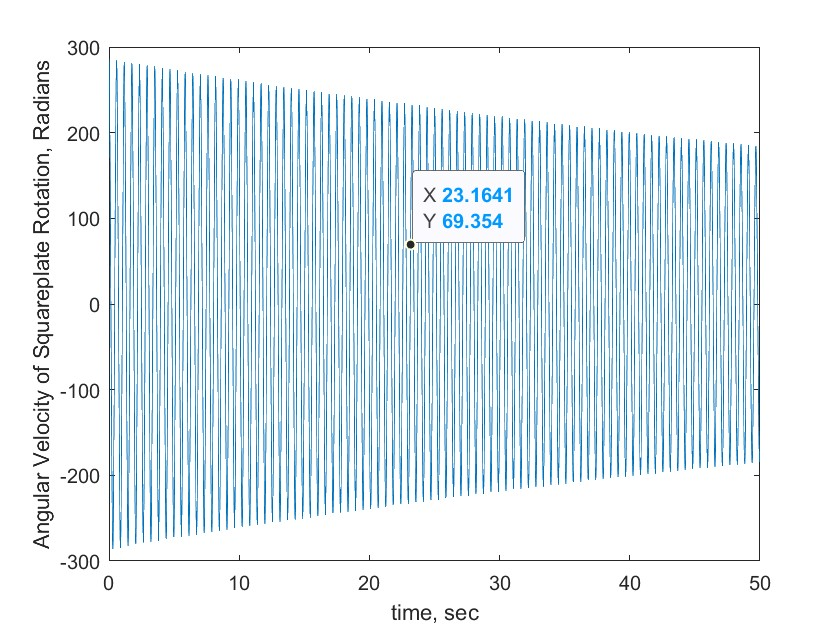
\includegraphics[scale=0.5]{images/phid_case_1.jpg}
    \caption{$\dot\phi$ for initial rotation of the square plate}
    \label{fig:phid_case1}
\end{figure}
and this for theta:
\begin{figure}[ht]
    \centering
    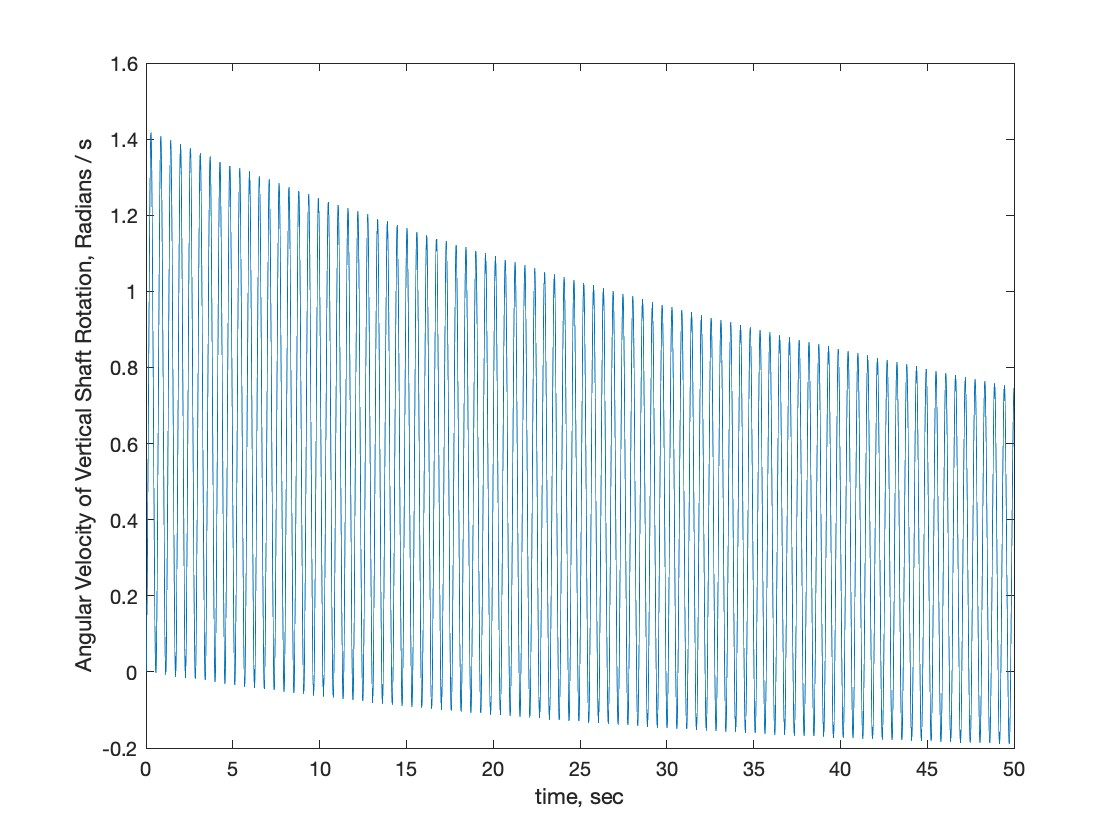
\includegraphics[scale=0.5]{images/thetad_case_1.jpg}
    \caption{$\dot\theta$ for initial rotation of the square plate}
    \label{fig:thetad_case1}
\end{figure}

And for the second initial conditions of exciting the theta around the vertical shaft:


\begin{equation}
    \begin{split}
        \begin{pmatrix}
            \dot \phi\\
            \dot \theta\\
            \phi\\
            \theta
        \end{pmatrix} = \begin{pmatrix}
            0\\
            5 s^{-1}\\
            0\\
            0
        \end{pmatrix}
    \end{split}
\end{equation}

we get for phi:
\begin{figure}[ht]
    \centering
    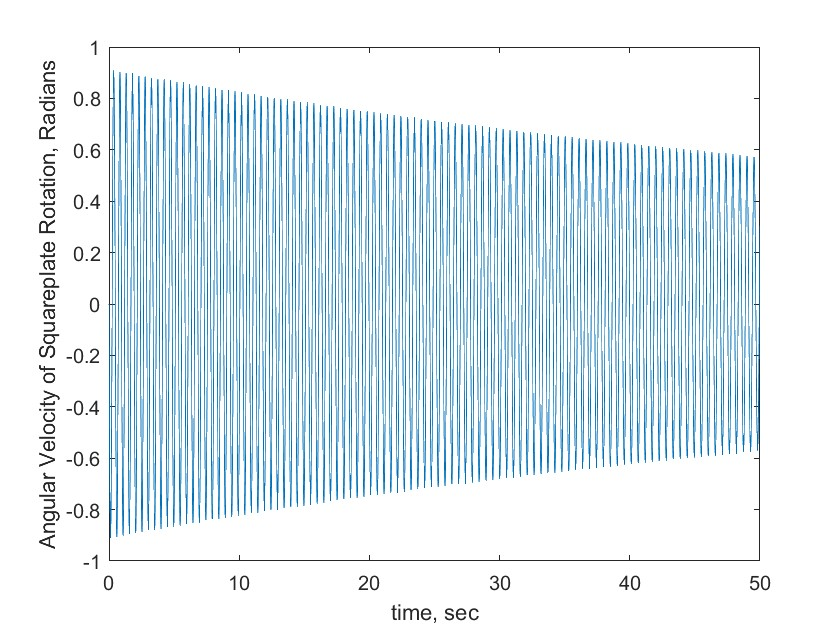
\includegraphics[scale=0.5]{images/phid_case_2.jpg}
    \caption{$\dot\phi$ for initial rotation of the vertical shaft}
    \label{fig:phid_case2}
\end{figure}
and for theta:
\begin{figure}[ht]
    \centering
    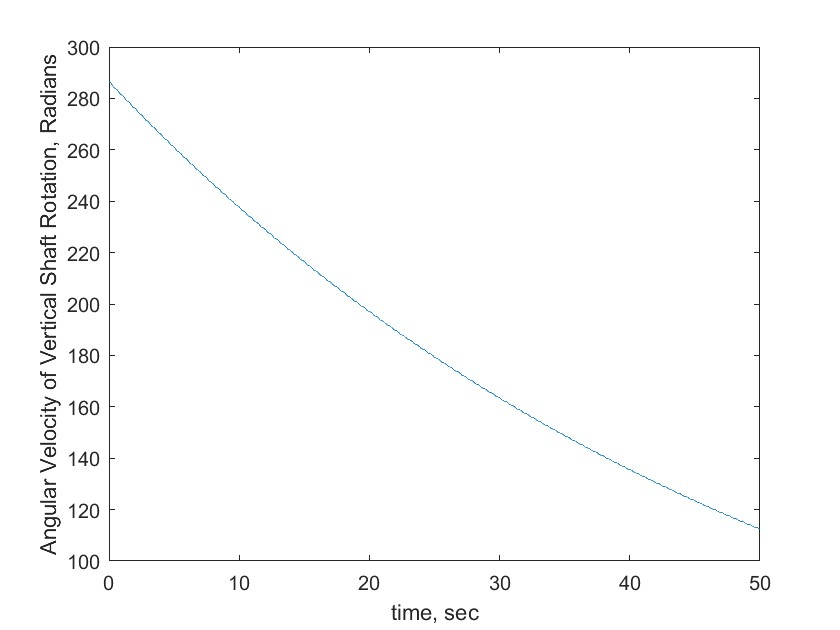
\includegraphics[scale=0.5]{images/thetad_case_2.jpg}
    \caption{$\dot\theta$ for initial rotation of the vertical shaft}
    \label{fig:thetad_case2}
\end{figure}